% CVPR 2026 Paper Template; see https://github.com/cvpr-org/author-kit

\documentclass[10pt,twocolumn,letterpaper]{article}

%%%%%%%%% PAPER TYPE  - PLEASE UPDATE FOR FINAL VERSION
% \usepackage{cvpr}              % To produce the CAMERA-READY version
\usepackage[review]{cvpr}      % To produce the REVIEW version
% \usepackage[pagenumbers]{cvpr} % To force page numbers, e.g. for an arXiv version

% Import additional packages in the preamble file, before hyperref
%% This file contains a number of tweaks that are typically applied to the main document.
%% They are not enabled by default, but can be enabled by uncommenting the relevant lines.


%%
%% NOTE: `cuted` is deliberately *not* loaded.  It redefines the output routine
%% to implement the `strip` environment (used only by the optional two-column
%% teaser, which is disabled in main.tex).  With it loaded, `strip` printed the
%% full-width qualitative figure past the bottom of the text block and on top of
%% the caption of another figure.  Re-enable it only together with fig/teaser.tex.
%%
% \usepackage{cuted} %< for the strip environment (two-column teaser only)

%%
%% Indent the first paragraph after section and subsection headings.
%%
\usepackage{indentfirst}
\setlength{\parindent}{1em}

%%
%% Keep bibliography entries compact. The CVPR style uses stretchable
%% bibliography spacing, which can expand excessively after a forced page break.
%%
\setlength{\bibsep}{1pt}

%%
%% For auto-referencing of figures (see fig/teaser.tex and \label{} therein) 
%%
\usepackage{currfile} %< for \currfilebase macro

%%
%% caption and (global) spacing overrides
%%
\usepackage{caption} %< for "\captionof" commands (teaser)
% Do not load the float package for forced [H] placement.  Standard LaTeX
% floating keeps figures and tables balanced across the two-column CVPR layout.
% \setlength{\abovecaptionskip}{.5em} % space above caption
% \setlength{\belowcaptionskip}{1em} % space below caption

%%
%% Inline annotations; for predefined colors, refer to "dvipsnames" in the xcolor package:
%% https://tinyurl.com/overleaf-colors
%%
\newcommand{\red}[1]{{\color{red}#1}}
\newcommand{\todo}[1]{{\color{red}#1}}
\newcommand{\TODO}[1]{\textbf{\color{red}[TODO: #1]}}
%%
%% Disable for camera ready / submission by uncommenting these lines:
%%
% \renewcommand{\TODO}[1]{}
% \renewcommand{\todo}[1]{#1}

%%
%% Work harder in optimizing text layout. Typically shrinks text by 1/6 of page, enable
%% it at the very end of the writing process, when you are just above the page limit.
%% (Measured on this draft: 12 pages either way, slightly tighter margins with it on.)
%%
% \usepackage{microtype}

%%
%% Fine-tune paragraph spacing.
%%
% \renewcommand{\paragraph}[1]{\vspace{.5em}\noindent\textbf{#1.}}

%%
%% Globally adjusts space between figure and caption.
%%
% \setlength{\abovecaptionskip}{.5em}

%%
%% Allows "the use of \paper to refer to the project name"
%% with automatic management of space at the end of the word.
%%
% \usepackage{xspace}
% \newcommand{\paper}{ProjectName\xspace}

%%
%% Commonly used math definitions.
%%
% \DeclareMathOperator*{\argmin}{arg\,min}
% \DeclareMathOperator*{\argmax}{arg\,max}

%%
%% Tighten underline.
%%
% \usepackage{soul}
% \setuldepth{foobar}

%%
%% Reconfigure paragraph (tweaks spacing)
%%


% It is strongly recommended to use hyperref, especially for the review version.
% hyperref with option pagebackref eases the reviewers' job.
% Please disable hyperref *only* if you encounter grave issues, 
% e.g. with the file validation for the camera-ready version.
%
% If you comment hyperref and then uncomment it, you should delete *.aux before re-running LaTeX.
% (Or just hit 'q' on the first LaTeX run, let it finish, and you should be clear).
\definecolor{cvprblue}{rgb}{0.21,0.49,0.74}
\usepackage[pagebackref,breaklinks,colorlinks,allcolors=cvprblue]{hyperref}

%%%%%%%%% PAPER ID  - PLEASE UPDATE
\def\paperID{*****} % *** Enter the Paper ID here
\def\confName{CVPR}
\def\confYear{2026}

%%%%%%%%% TITLE - PLEASE UPDATE
\title{Trust What You Transfer: Knowledge-Enhanced Hard-Soft Reasoning for Cross-Domain Few-Shot Object Detection}

%%%%%%%%% AUTHORS - PLEASE UPDATE
\author{First Author\\
Institution1\\
Institution1 address\\
{\tt\small firstauthor@i1.org}
% For a paper whose authors are all at the same institution,
% omit the following lines up until the closing ``}''.
% Additional authors and addresses can be added with ``\and'',
% just like the second author.
% To save space, use either the email address or home page, not both
\and
Second Author\\
Institution2\\
First line of institution2 address\\
{\tt\small secondauthor@i2.org}
}

\begin{document}
\maketitle
% Optional first-page teaser. Uncomment after placing the figure in fig/teaser.pdf.
% \begin{strip}
\centering
\includegraphics[width=.33\linewidth]{example-image-golden}\hfill
\includegraphics[width=.33\linewidth]{example-image-golden}\hfill
\includegraphics[width=.33\linewidth]{example-image-golden}
\captionsetup{hypcap=false}
\captionof{figure}{\textbf{Teaser} -- example of a 2-column teaser. This figure appears at the top of the first page, and a two-column teaser is not mandatory.}
\captionsetup{hypcap=true}
\label{fig:\currfilebase}%
\end{strip}
\begin{abstract}
Cross-domain few-shot object detection (CD-FSOD) adapts a pretrained detector to unseen domains using only a few labeled examples. Existing methods transfer visual prototypes, generated data, or multimodal prompts, but often treat every support factor as valid adaptation evidence. We identify \emph{support-induced context leakage}: changing only the support background can alter query classification and localization, even when the query image and support foreground remain fixed. We propose a knowledge-enhanced Hard-Soft framework that regulates both the evidence being transferred and its authority over model decisions. Foreground-Frozen Context Probing (FFCP) estimates class-wise context-sensitive subspaces through label-preserving support interventions. Context-Constrained Hard-Soft Decomposition (CHSD) constructs a Hard identity anchor and a reliability-weighted Soft target-domain prototype after removing context-sensitive directions. Asymmetric Task-Authority Routing (ATAR) uses Hard--Soft agreement as a reliability signal and applies a bounded cosine correction only to uncertain detector queries. The correction is zero at initialization and leaves the localization branch unchanged. The full model, denoted S2H-CD-FSOD, is evaluated on six CD-FSOD benchmarks under 1-, 5-, and 10-shot protocols. A controlled study on Clipart1k and NEU-DET separates context-induced category and box drift from training-seed variation, and a compact set of ablations and qualitative comparisons clarifies when support evidence helps and when its authority should be suppressed.
\end{abstract}

\begin{figure}[t]
    \centering
    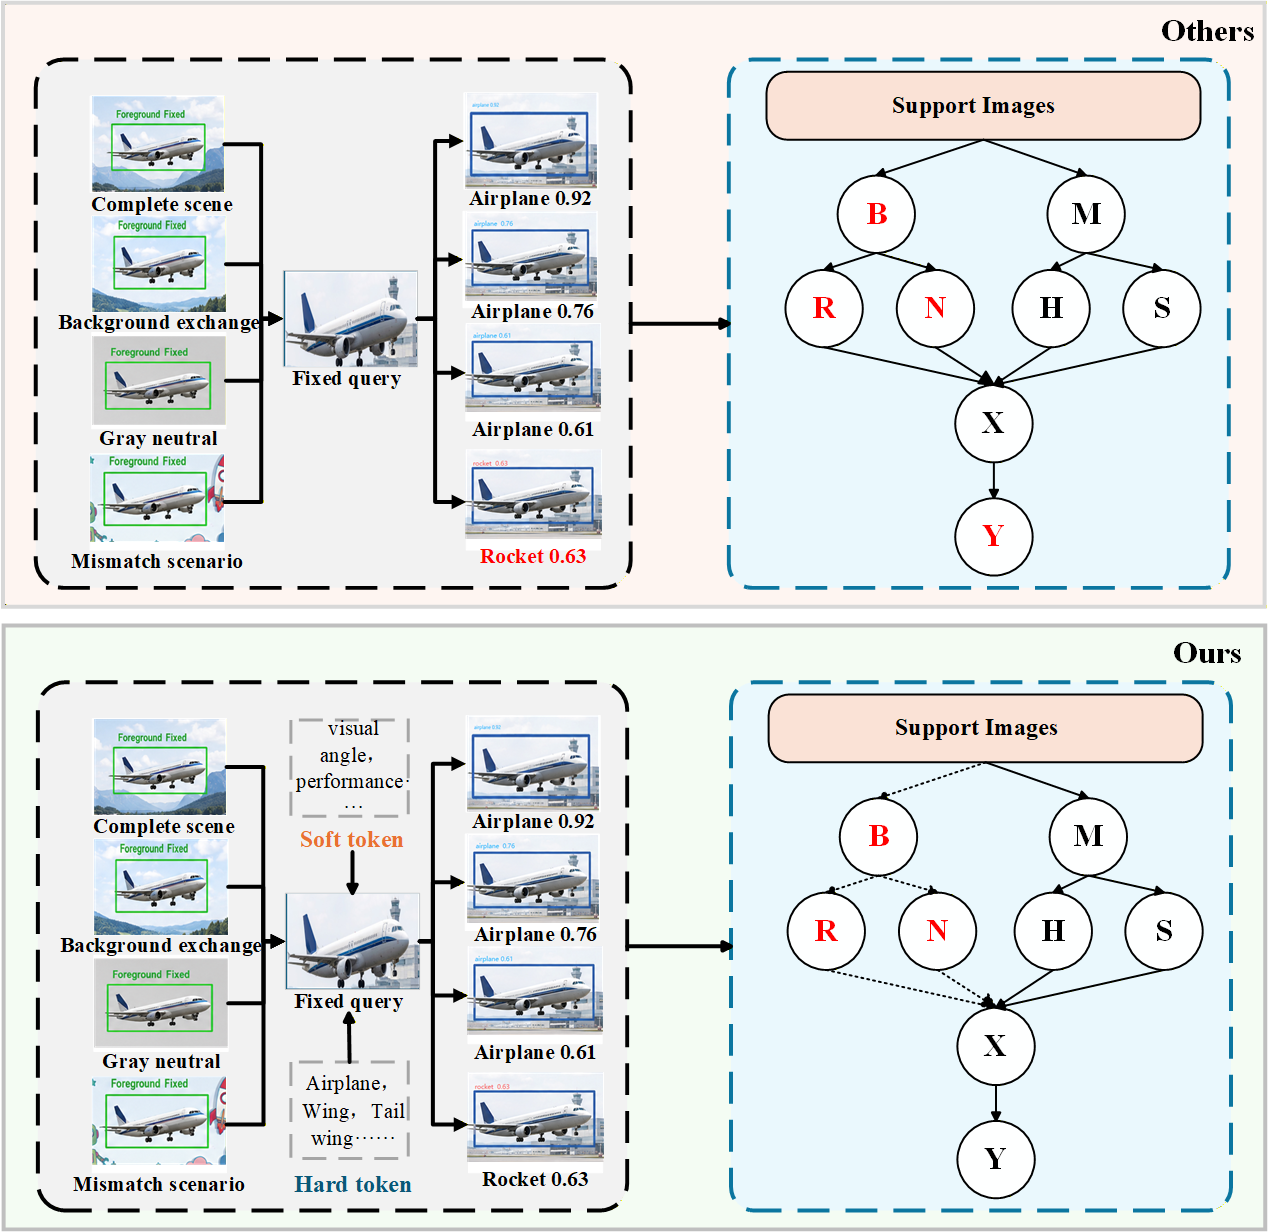
\includegraphics[width=\linewidth]{fig/context_leakage.png}
    \caption{\textbf{Motivation: support-induced context leakage.} \textbf{Top:} treating every support factor as valid evidence lets category-irrelevant context reach the query decision. With the support foreground, box, and query fixed, changing only the support context already shifts the confidence and, in the last row, the predicted category. \textbf{Bottom:} our framework separates category identity from domain appearance. A Hard token carries context-invariant identity, a Soft token carries only context-cleaned target appearance, and the authority routing decides how far either token may move the decision. Solid and dashed arrows denote retained and suppressed influences.}
    \label{fig:context-leakage}
\end{figure}

\section{Introduction}
\label{sec:intro}

Pretraining on large-scale vision and vision-language data has substantially improved object detection~\cite{detr,dino,groundingdino}. Nevertheless, detectors trained on natural images remain brittle in aerial, industrial, underwater, and artistic domains, which differ in viewpoint, scale, texture, illumination, and scene composition. Because dense annotation in these domains is expensive, cross-domain few-shot object detection (CD-FSOD) seeks to adapt a source-pretrained detector using only a few labeled examples per category~\cite{cdvito,domainrag}.

Recent work employs feature caching and sparse adaptation~\cite{ifc,sivito}, augmentation and retrieval-guided generation~\cite{ets,domainrag}, foundation-model experts~\cite{vfmmoe,yu2026}, or multimodal prototypes and visual prompts~\cite{lmp,petdino,astigmatism}. These methods share a common premise: scarce target examples contain useful domain evidence. This premise, however, is incomplete. A support image contains category identity, relevant foreground appearance, and incidental scene context. A DIOR airplane, for example, provides a useful near-nadir silhouette and small-object texture, but may also appear alongside runways or buildings that do not define the category. A mixed prototype can improve domain alignment while allowing such incidental context to shift the pretrained category boundary.

We investigate this failure mode through the controlled intervention shown in Fig.~\ref{fig:context-leakage}. We preserve the support foreground, bounding box, scale, and query set, changing only the pixels outside a protected support region. Across Clipart1k and NEU-DET, this intervention alters category distributions and predicted boxes beyond the variation induced by training seeds. We refer to this phenomenon as \emph{support-induced context leakage}. Its severity is domain dependent: neutralization is the most disruptive intervention for several NEU-DET diagnostics, whereas mismatched context causes the clearest aggregate degradation on Clipart1k. Context sensitivity therefore reflects the interaction among support evidence, domain statistics, and detector adaptation, rather than a fixed ranking of corruption severity.

This observation shifts the adaptation question from \emph{how much target knowledge can be injected?} to \emph{when should target knowledge be allowed to alter a decision?} We address this question with the knowledge-enhanced Hard-Soft framework illustrated in Fig.~\ref{fig:overview}. Foreground-Frozen Context Probing (FFCP) estimates where and to what extent context enters each category representation. Context-Constrained Hard-Soft Decomposition (CHSD) constructs a Hard identity anchor and a reliability-weighted Soft target-domain prototype after removing context-sensitive directions from the original support foreground. Asymmetric Task-Authority Routing (ATAR) uses agreement between these two estimates to determine prototype reliability, then applies a bounded cosine correction only to uncertain Grounding DINO queries. The framework retains a single detector and preserves its original localization path.

We evaluate the resulting method across six target domains and three shot regimes. Beyond aggregate detection accuracy, we measure fixed-query context sensitivity and inspect whether improvements arise from reduced background responses or from indiscriminate score changes. The method does not discard target-domain evidence; it preserves useful foreground variation while restricting unsupported category corrections.

Our contributions are summarized as follows:
\begin{itemize}
    \item We identify support-induced context leakage and introduce a foreground-preserving, fixed-query protocol that separates context effects from ordinary training-seed variation, verifying the phenomenon in both artistic and industrial target domains.
    \item We propose FFCP and CHSD to estimate context-sensitive directions and sequentially decompose support evidence into bounded Hard identity knowledge and context-cleaned Soft appearance knowledge.
    \item We introduce ATAR, a reliability-constrained Grounding DINO interface that uses Hard--Soft agreement and query uncertainty to bound class-score correction while preserving the baseline localization path. We evaluate its accuracy and context robustness across six CD-FSOD benchmarks.
\end{itemize}

\section{Related Work}
\label{sec:related}

\subsection{Few-Shot and Cross-Domain Detection}

Few-shot object detection learns novel categories from scarce annotations. Early meta-learning approaches condition a detector on support features, whereas transfer-learning methods show that carefully constrained fine-tuning can be surprisingly competitive. Representative methods include TFA~\cite{tfa}, FSCE~\cite{fsce}, and DeFRCN~\cite{defrcn}, which study restricted classifier adaptation, contrastive proposal representations, and decoupled classification and localization, respectively. These methods generally assume that base and novel data originate from the same domain.

CD-FSOD further introduces a severe source--target domain shift. CD-ViTO~\cite{cdvito} established a six-domain benchmark and enhanced an open-set detector with target instances. Subsequent work caches target features~\cite{ifc}, searches for foundation-model augmentations~\cite{ets}, retrieves compositional data~\cite{domainrag}, or exploits style augmentation and sparse target instances~\cite{styleproto,sivito}. VFM-MoE~\cite{vfmmoe} combines DETR with foundation-model experts, while Yu \etal~\cite{yu2026} show that progressive schedules and decoder diversity are critical to stable few-shot fine-tuning. Target-Domain Astigmatism~\cite{astigmatism}, in contrast, diagnoses dispersed attention and refines both foreground and peripheral context. Our work is complementary to these approaches: we examine whether each support-derived factor receives decision authority commensurate with its reliability.

\subsection{Vision-Language Detectors and Support Knowledge}

Open-vocabulary detectors transfer category semantics by aligning visual regions with language. Representative directions include region-text knowledge distillation in ViLD~\cite{vild}, region-level language-image pretraining in RegionCLIP~\cite{regionclip}, end-to-end multimodal decoding in MDETR~\cite{mdetr}, conditional matching in OV-DETR~\cite{ovdetr}, and image-text prompting in OWL-ViT~\cite{owlvit}. On the detection side, Deformable DETR~\cite{deformable_detr}, DAB-DETR~\cite{dab_detr}, and DN-DETR~\cite{dn_detr} improve the convergence and query design of the original DETR formulation~\cite{detr}. GLIP~\cite{glip} formulates detection as phrase grounding, while Grounding DINO~\cite{groundingdino} combines encoder-level feature fusion, language-guided query selection, and cross-modal decoder interaction with the DINO detector~\cite{dino}. Such models provide strong initializations for CD-FSOD because category names remain meaningful across domains; however, text alone cannot capture target-specific appearance.

Recent methods therefore inject visual support knowledge. LMP~\cite{lmp} constructs class prototypes and query-derived hard negatives in a visual branch, while PET-DINO~\cite{petdino} unifies instance- and category-level visual cues through prompt-enriched training. Target-Domain Astigmatism~\cite{astigmatism} jointly models foreground prototypes, contextual background, and text. These approaches demonstrate that support features can complement language, but they typically optimize each prototype as a complete representation. In contrast, CHSD distinguishes the component that defines category identity from the component that captures necessary domain appearance. ATAR further controls the stage at which, and the magnitude with which, each component enters the detector.

\subsection{Context Sensitivity and Prediction Reliability}

Context can support object-boundary estimation and category disambiguation, yet it can also become a shortcut that produces background false positives under distribution shift. Existing CD-FSOD methods use negative regions as contrastive cues~\cite{lmp}, explicitly model peripheral background~\cite{astigmatism}, or evaluate robustness on mixed-domain queries~\cite{yu2026}. Confidence calibration offers a complementary perspective: a detector should not only be accurate, but also align confidence with correctness and identify high-risk predictions~\cite{calibration,selective}.

Our focus differs in two respects. First, we intervene on the support set rather than the query: the query remains fixed while the context outside the protected support foreground changes. Second, the intervention serves as a diagnostic probe rather than as additional labeled data. FFCP measures prediction drift across support conditions, CHSD excludes context-sensitive directions from target-appearance knowledge, and ATAR contracts Soft classification authority when support evidence is unstable. Together, these modules connect support-side sensitivity to detection accuracy, calibration, and selective risk.

\begin{figure*}[t]
    \centering
    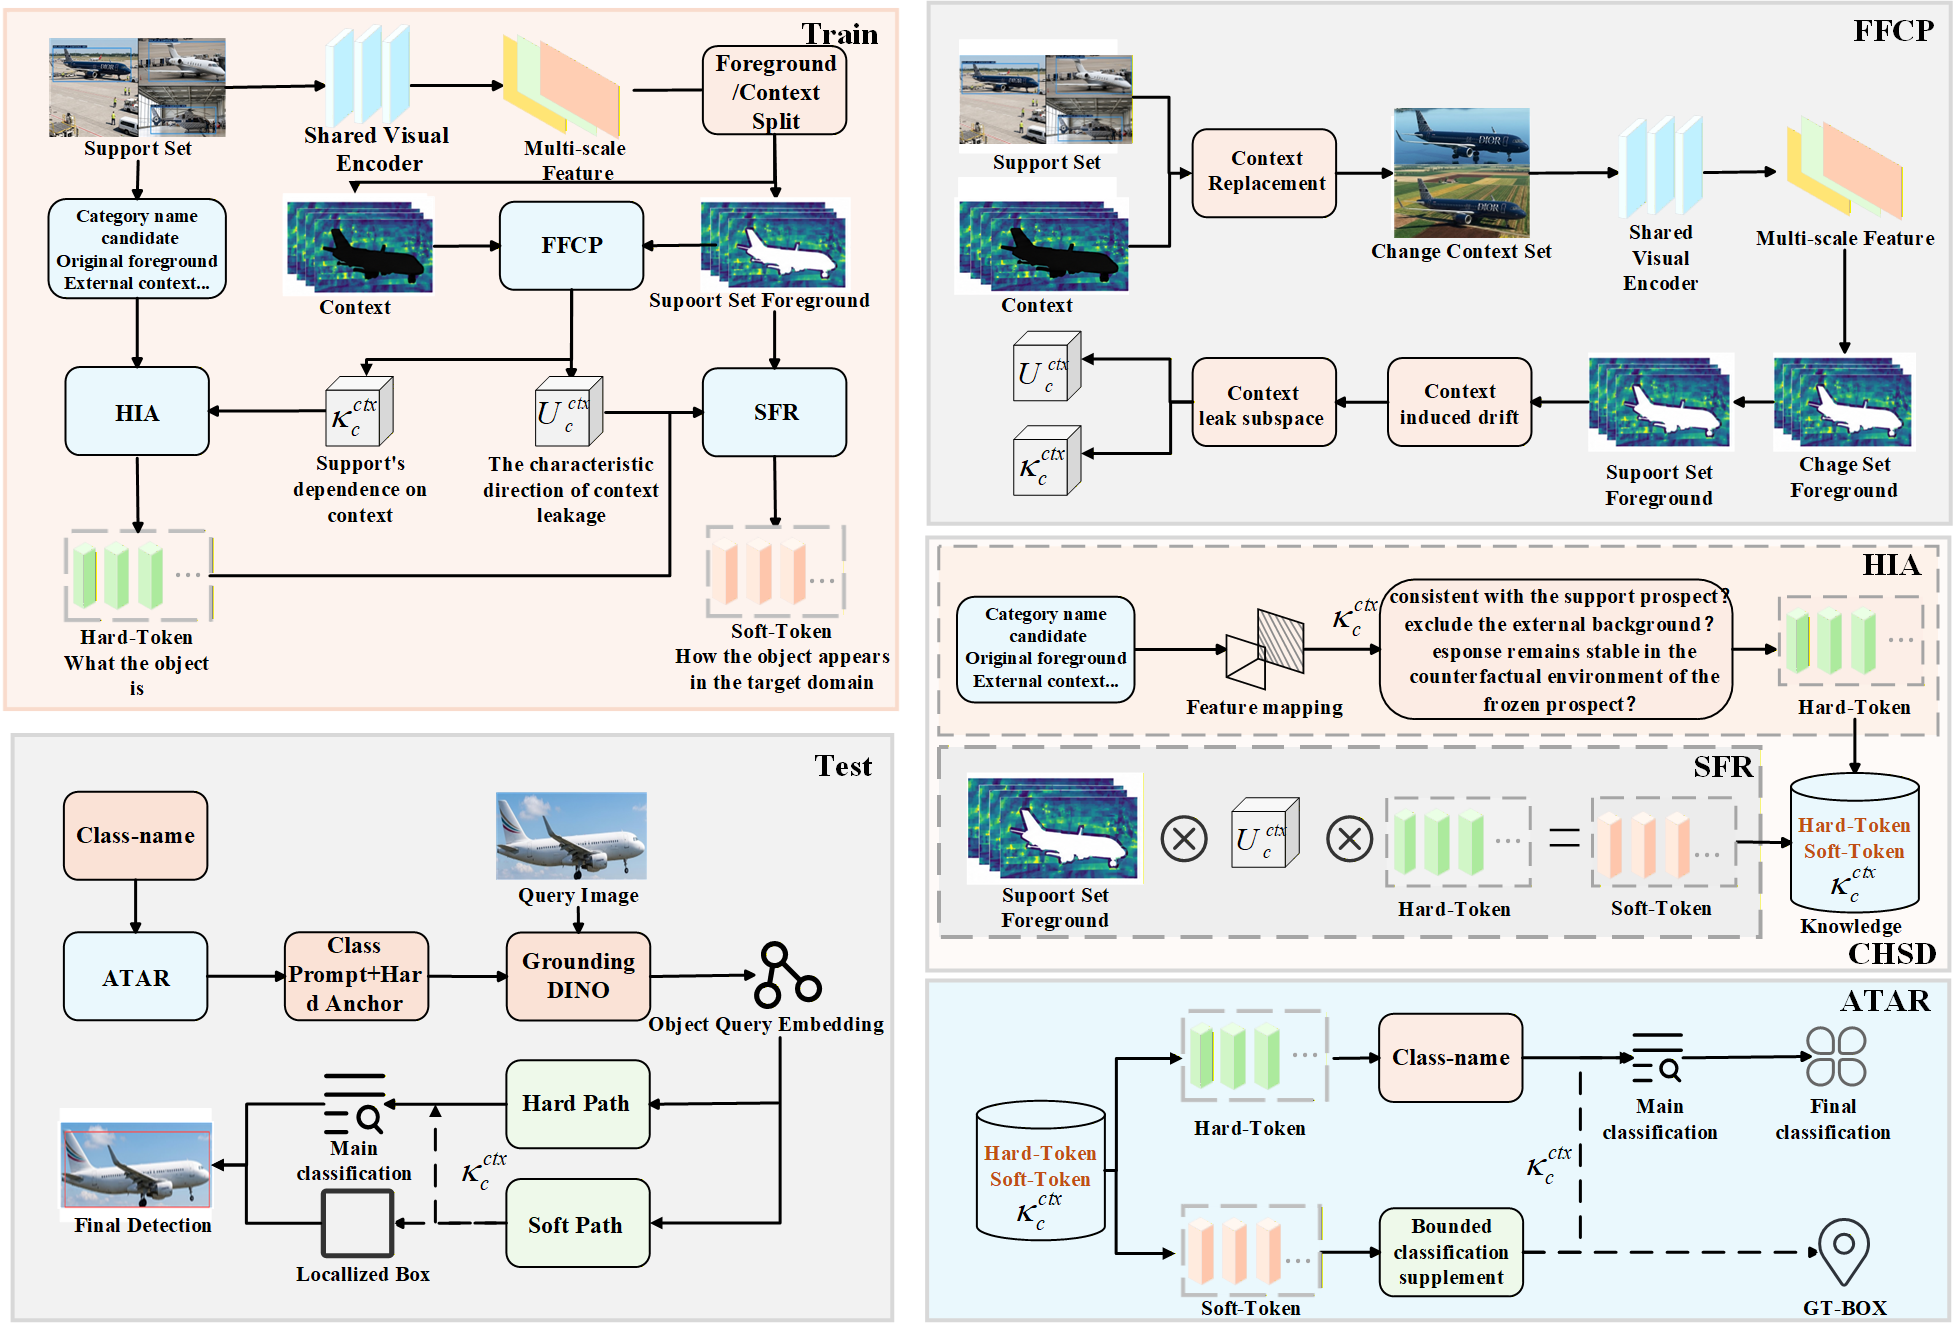
\includegraphics[width=\textwidth]{fig/method_overview.png}
    \caption{\textbf{Knowledge-enhanced Hard--Soft framework.} (1) Foreground-Frozen Context Probing (FFCP) modifies only the support context and estimates a class-wise context-sensitive subspace. (2) Context-Constrained Hard--Soft Decomposition (CHSD) builds a bounded Hard identity anchor and a context-cleaned Soft appearance residual. (3) Grounding DINO first produces its ordinary query predictions. (4) Asymmetric Task-Authority Routing (ATAR) uses Hard--Soft agreement and baseline-query uncertainty to authorize a bounded cosine class correction while leaving the localization output unchanged.}
    \label{fig:overview}
\end{figure*}


\section{Method}
\label{sec:method}

Figure~\ref{fig:overview} presents our knowledge-enhanced Hard-Soft framework. We formulate target-domain adaptation as a constrained knowledge update rather than a complete prototype transfer. Foreground-Frozen Context Probing (FFCP) measures how support context perturbs an otherwise unchanged foreground representation. Context-Constrained Hard-Soft Decomposition (CHSD) then constructs a Hard identity anchor and a reliability-weighted, context-cleaned Soft prototype. Finally, Asymmetric Task-Authority Routing (ATAR) uses Hard--Soft agreement and baseline-query uncertainty to bound a cosine class correction in a single Grounding DINO detector~\cite{groundingdino}. Hard knowledge controls whether the Soft direction is trustworthy; it is not injected as an independent classifier, and the baseline localization path remains unchanged. We refer to the complete instantiation as S2H-CD-FSOD.

\subsection{Preliminaries}
\label{sec:preliminaries}

Let $\mathcal C$ denote the target-category set. Following standard CD-FSOD protocols~\cite{cdvito,yu2026}, the support set of category $c$ and the predictions for an unlabeled query image $x_q$ are
\begin{equation}
\begin{aligned}
\mathcal S_c^K
&=\{(x_{c,i},b_{c,i},c)\}_{i=1}^{K},
\quad K\in\{1,5,10\},\\
\widehat{\mathcal Y}_q
&=\{(\hat b_j,\hat y_j,\hat p_j)\}_{j=1}^{M'}.
\end{aligned}
\label{eq:problem}
\end{equation}
where $x_{c,i}$ and $b_{c,i}$ denote a support image and its annotated bounding box, respectively. At inference time, neither query boxes nor query labels are available. Category names are obtained from the support annotations and used to form the textual prompt, but support knowledge never directly assigns a label to a query object.

Grounding DINO aligns image regions with textual phrases and performs language-guided query selection before Transformer decoding~\cite{groundingdino}. We keep this open-vocabulary path unchanged and apply support calibration only after the ordinary decoder logits are available. For each category, our support-side procedure constructs
\begin{equation}
\mathcal K_c=(\mathbf h_c,\mathbf s_c,
\kappa_c^{\mathrm{ctx}}),
\label{eq:knowledge_cache}
\end{equation}
where $\mathbf h_c$ is the Hard identity anchor, $\mathbf s_c$ denotes Soft foreground-appearance knowledge, and $\kappa_c^{\mathrm{ctx}}\in[0,1)$ measures the dependence of the support representation on external context.

\subsection{Foreground-Frozen Context Probing}
\label{sec:ffcp}

Although support features are pooled from annotated boxes, the visual encoder can still transmit information from runways, water, roads, or industrial substrates. FFCP estimates this influence through foreground-preserving interventions. We dilate each support box to obtain a protection mask $M_{c,i}$ that covers the target and its boundary. The $r$-th intervened support image is
\begin{equation}
\tilde x_{c,i}^{(r)}
=M_{c,i}\odot x_{c,i}
+(1-M_{c,i})\odot B_i^{(r)},
\label{eq:counterfactual}
\end{equation}
where $B_i^{(r)}$ is obtained through in-domain background exchange, category-mismatched exchange, or context neutralization. The protected pixels, box geometry, viewpoint, scale, resolution, and foreground texture remain unchanged. These intervened views serve only as probes and are never counted as additional shots.

The original image, its intervened counterpart, and a reconstruction control are processed by the same frozen visual encoder. RoIAlign and attention pooling extract the target representations $\mathbf f_{c,i}$, $\tilde{\mathbf f}_{c,i}^{(r)}$, and $\mathbf f_{c,i}^{\mathrm{rec}}$ from the same box. The reconstruction control uses the same synthesis pipeline but reinserts the original context. We define the resulting context-induced drift as
\begin{equation}
\mathbf d_{c,i}^{(r)}
=\big(\mathbf f_{c,i}-\tilde{\mathbf f}_{c,i}^{(r)}\big)
-\big(\mathbf f_{c,i}-\mathbf f_{c,i}^{\mathrm{rec}}\big),
\label{eq:context_drift}
\end{equation}
The second term removes drift caused by compositing and resampling. A nonzero residual indicates that external context perturbs the protected target representation.

Let $\mathbf D_c$ stack all drift vectors for category $c$. We retain its leading right-singular vectors and quantify the normalized leakage energy as
\begin{equation}
\begin{aligned}
\mathbf U_c^{\mathrm{ctx}}
&=\operatorname{TopSVD}(\mathbf D_c,r),\\
e_c^{\mathrm{ctx}}
&=\frac{1}{KR}\sum_{i,r}
\frac{\|({\mathbf U_c^{\mathrm{ctx}}})^\top
\mathbf d_{c,i}^{(r)}\|_2^2}
{\|\mathbf f_{c,i}\|_2^2+\epsilon},\\
\kappa_c^{\mathrm{ctx}}
&=1-\exp(-e_c^{\mathrm{ctx}}).
\end{aligned}
\label{eq:context_subspace}
\end{equation}
The columns of $\mathbf U_c^{\mathrm{ctx}}$ describe \emph{where} context enters the target representation, while $\kappa_c^{\mathrm{ctx}}$ quantifies \emph{how strongly} the support depends on context. For 1-shot adaptation, we restrict the rank and shrink the class-specific estimate toward a cross-category drift subspace. As $K$ increases, the class-specific estimate receives greater weight.

\subsection{Context-Constrained Hard-Soft Decomposition}
\label{sec:chsd}

FFCP identifies context-sensitive directions but does not determine category identity. CHSD therefore decomposes support knowledge in two stages: it first identifies invariant category factors and then extracts adaptable target-domain appearance.

For category $c$, we obtain a compact candidate set from its name, synonyms, and deterministic structural attributes. For example, valid identity hypotheses for an airplane include wings, a fuselage, and a tail, but exclude a top-down view, low resolution, or a runway. These candidates are drawn from predefined structural templates rather than free-form target-domain generation. Recent CD-FSOD methods have demonstrated that support prototypes can complement pretrained textual semantics~\cite{lmp,astigmatism}; CHSD additionally determines whether each candidate is sufficiently reliable to alter category knowledge. After mapping the textual and visual features into the normalized Grounding DINO alignment space, we measure counterfactual instability and define the qualification score for attribute $\mathbf a_{c,l}$ as
\begin{equation}
\begin{aligned}
\Delta_{c,l}^{\mathrm{cf}}
&=\frac{1}{KR}\sum_{i,r}
\left|
\operatorname{sim}(\mathbf a_{c,l},\mathbf f_{c,i})
-\operatorname{sim}(\mathbf a_{c,l},
\tilde{\mathbf f}_{c,i}^{(r)})
\right|,\\
q_{c,l}={}&
\operatorname{sim}(\mathbf a_{c,l},\bar{\mathbf f}_c^{\mathrm{fg}})
-\lambda_b
\big[\operatorname{sim}(\mathbf a_{c,l},
\bar{\mathbf f}_c^{\mathrm{ctx}})\big]_+\\
&-\lambda_{\mathrm{cf}}\Delta_{c,l}^{\mathrm{cf}}
-\lambda_\kappa\kappa_c^{\mathrm{ctx}}.
\end{aligned}
\label{eq:hard_qualification}
\end{equation}
The four terms enforce foreground support, reject positive context correlation, penalize intervention-sensitive attributes, and reduce the qualification scores of categories whose support is globally context dependent, respectively. Thus, $\kappa_c^{\mathrm{ctx}}$ influences Hard construction rather than being used only at query time.

Only candidates whose scores exceed the threshold $\xi_H$ are retained. Their weighted aggregate is projected onto an $\ell_2$ ball before being added to the base category embedding $\mathbf t_c^0$:
\begin{equation}
\begin{aligned}
\mathcal V_c&=\{l\mid q_{c,l}\geq\xi_H\},\qquad
w_{c,l}=\operatorname{softmax}_{l\in\mathcal V_c}
(q_{c,l}/T_q),\\
\Delta\mathbf h_c
&=\Pi_{\|\cdot\|_2\leq\rho_H}
\left(\sum_{l\in\mathcal V_c}w_{c,l}\mathbf a_{c,l}\right),\\
\mathbf h_c&=\operatorname{Norm}
(\mathbf t_c^0+\Delta\mathbf h_c).
\end{aligned}
\label{eq:hard_anchor}
\end{equation}
If no attribute qualifies, we set $\Delta\mathbf h_c=\mathbf 0$ and recover the original category representation. The radius $\rho_H$ prevents a few support instances from arbitrarily rewriting pretrained category semantics.

Hard knowledge should not absorb target-domain appearance factors such as nadir viewpoints, compressed scale, blur, or low-resolution texture. We map the base identity and accepted attributes into the visual space and orthonormalize them to obtain the identity subspace $\mathbf U_c^H$. We remove context leakage only within the identity complement, thereby preventing context suppression from erasing category-defining directions. The Soft residual for support instance $i$ is
\begin{equation}
\begin{aligned}
\mathbf P_c^H&=\mathbf U_c^H({\mathbf U_c^H})^\top,\\
\bar{\mathbf U}_c^{\mathrm{ctx}}
&=\operatorname{Orth}\!\left[
(\mathbf I-\mathbf P_c^H)\mathbf U_c^{\mathrm{ctx}}
\right],\\
\mathbf r_{c,i}^{\mathrm{app}}
&=(\mathbf I-\mathbf P_c^H)
\left(\mathbf I-\bar{\mathbf U}_c^{\mathrm{ctx}}
({\bar{\mathbf U}_c^{\mathrm{ctx}}})^\top\right)
\mathbf f_{c,i}.
\end{aligned}
\label{eq:soft_residual}
\end{equation}
Counterfactual background features never enter Soft knowledge. FFCP identifies the directions to be removed, whereas the retained appearance is always derived from the original support foreground.

We robustly aggregate the residuals and apply shot-aware shrinkage:
\begin{equation}
\mathbf s_c=(1-\alpha_K)
\operatorname{RobustMean}
\big(\{\mathbf r_{c,i}^{\mathrm{app}}\}_{i=1}^{K}\big),
\qquad
\alpha_K=\frac{\xi}{K+\xi}.
\label{eq:soft_aggregation}
\end{equation}
This estimator remains conservative in the 1-shot setting and places progressively greater trust in the target-domain residual as more support instances become available. It changes only the stability of knowledge estimation; the network architecture remains identical across the 1-, 5-, and 10-shot protocols.

\subsection{Asymmetric Task-Authority Routing}
\label{sec:atar}

ATAR connects the support-side decomposition to query detection without
granting a noisy few-shot prototype unrestricted authority. Grounding DINO
first produces decoded query embeddings $\mathbf z_j$, boxes $\mathbf b_j$,
and category logits $L^0_{j,c}$ from the ordinary textual prompts. The Hard
anchor is used as a reliability signal rather than being injected into the
text or added directly to the logits. This preserves the pretrained
vision--language boundary and lets support knowledge act only through a
bounded calibration interface.

For category $c$, CHSD supplies a prototype reliability $r_c\in[0,1]$. We
further measure the agreement between the Soft prototype and the Hard anchor:
\begin{equation}
q_c=\frac{1+\operatorname{cos}(\mathbf s_c,\mathbf h_c)}{2},
\qquad \bar r_c=r_c q_c.
\label{eq:hard_reliability}
\end{equation}
Thus, Hard knowledge does not vote for a class; it determines how much the
corresponding Soft direction may be trusted. When the two support estimates
disagree, the calibration authority contracts automatically.

We next restrict correction to uncertain detector queries. Let
$p_j^0=\max_c\sigma(L^0_{j,c})$. The query authority is
\begin{equation}
u_j=\sigma\!\left(\frac{\theta-p_j^0}{T_u}\right),
\qquad
g_{j,c}=\min(u_j\bar r_c,g_{\max}),
\label{eq:query_authority}
\end{equation}
where $\theta$, $T_u$, and $g_{\max}$ are fixed threshold, temperature, and
authority ceiling. Confident baseline queries receive almost no update,
whereas uncertain queries can consult reliable target-domain evidence.

Finally, the class correction follows the Soft prototype direction:
\begin{equation}
\begin{aligned}
d_{j,c}&=\operatorname{cos}(\mathbf z_j,\mathbf s_c),\\
\delta_{j,c}&=\gamma g_{\mathrm{cls}}g_{j,c}\alpha_c d_{j,c},\\
L_{j,c}&=L^0_{j,c}+\delta_{j,c},
\quad
|\delta_{j,c}|\leq
\gamma g_{\mathrm{cls}}g_{\max}\alpha_{\max}.
\end{aligned}
\label{eq:soft_classification}
\end{equation}
Here $g_{\mathrm{cls}}$ is a learned sigmoid gate and
$\alpha_c\in[0,\alpha_{\max}]$ is a class-wise strength initialized to zero.
Consequently, the enhanced model is identical to the baseline at
initialization and can depart from it only along a class prototype direction.
The current model is classification-only: it retains Grounding DINO's box
prediction unchanged. This isolates the proposed reliability mechanism from
an additional localization adapter.

\subsection{Model Training and Testing}
\label{sec:training}

We retain the standard bipartite matching and detection objectives used by
DETR-family detectors~\cite{detr,dino,groundingdino}. Hungarian matching and
the phrase-level focal, $\ell_1$, and GIoU losses are unchanged. We add a
small residual penalty and distill the baseline category distribution on the
queries selected by Eq.~\eqref{eq:query_authority}:
\begin{equation}
\begin{aligned}
\mathcal L_{\mathrm{total}}={}&
\lambda_{\mathrm{cls}}\mathcal L_{\mathrm{focal}}^{\mathrm{phrase}}
+\lambda_1\mathcal L_1
+\lambda_g\mathcal L_{\mathrm{GIoU}}\\
&+\lambda_{\mathrm{res}}\|\boldsymbol\delta\|_1
+\lambda_{\mathrm{con}}
\frac{\sum_j u_jD_{\mathrm{KL}}(p_j^0\|p_j)}
{\sum_j u_j+\epsilon}.
\end{aligned}
\label{eq:total_loss}
\end{equation}
The first auxiliary term discourages unnecessary score changes; the second
prevents low-confidence calibration from destroying a useful baseline
ranking. At inference, the knowledge tuple in
Eq.~\eqref{eq:knowledge_cache} is built once and cached. Counterfactual views
are used only on the support side and never expose query labels or increase
the number of annotated instances.

\paragraph{Properties and scope.}
Under a local additive representation, the foreground-frozen difference
cancels identity and foreground appearance, while the reconstruction control
removes synthesis drift. Equation~\eqref{eq:soft_classification} gives an
explicit correction bound, and Eqs.~\eqref{eq:hard_reliability}--\eqref{eq:query_authority}
make that bound shrink with prototype disagreement and baseline confidence.
FFCP still assumes that the protection mask covers the discriminative target
and that compositing artifacts remain controlled; these assumptions are
examined through the controlled context study and supplementary sensitivity
analysis.

\section{Experiments}
\label{sec:experiments}

We organize the experiments to mirror this narrative: we first report a controlled support-context study that establishes the motivating phenomenon, then the main comparison against state-of-the-art methods across six domains, followed by the prototype-space and hyper-parameter analyses, and finally a component ablation that connects the quantitative gains to the per-stage behavior of the detector.

\subsection{Experimental Setup}
\label{sec:exp_setup}

\paragraph{Datasets.}
Following the established CD-FSOD benchmark~\cite{cdvito,astigmatism,lmp}, we evaluate our method on six target domains: ArTaxOr (photorealistic arthropods), Clipart1k (cartoon imagery), DIOR (aerial scenes), DeepFish (low-visibility aquatic imagery), NEU-DET (industrial defects), and UODD (underwater objects). These datasets contain 7, 20, 20, 1, 6, and 3 categories, respectively, and vary substantially in texture, scale, viewpoint, and background statistics.

\paragraph{Few-shot protocol.}
We report results for 1-, 5-, and 10-shot adaptation, using five deterministic support splits in each setting. All methods share the same category set, support splits, query images, optimization budget, and augmentation policy. We fix checkpoints and hyperparameters without using test annotations from the target domains. For the densely annotated DIOR dataset, we select $K$ support images per category and retain all annotations in their union, preventing co-occurring objects from being mislabeled as background. We evaluate every method under this image-level protocol, while the remaining datasets follow the standard $K$-instance protocol.

\paragraph{Metrics.}
We evaluate detection performance using COCO mAP over IoU thresholds from $0.50$ to $0.95$, AP50, AP75, and area-stratified AP. We quantify support sensitivity using classification and box Context Sensitivity Scores (CSS-cls and CSS-box), category flip rate, localization flip rate, and the number of background false positives. We assess confidence reliability using ECE~\cite{calibration}, negative log-likelihood (NLL), the Brier score, and the area under the risk--coverage curve (AURC)~\cite{selective}. Unless stated otherwise, all tables report the mean and sample standard deviation over five support splits.

\paragraph{Implementation details.}
We use Grounding DINO with a Swin-B image encoder and a BERT-base language encoder~\cite{groundingdino}. All variants are initialized from the public Swin-B checkpoint
\texttt{groundingdino\_swinb\allowbreak\_cogcoor\allowbreak\_mmdet-55949c9c.pth},
matching the Grounding DINO$^\dagger$ configuration used by Domain-RAG~\cite{domainrag}. We optimize with AdamW using a learning rate of $1\times10^{-4}$, weight decay of $1\times10^{-4}$, and a $0.1$ learning-rate multiplier for the image backbone. The training batch size is four and gradients are clipped to a maximum norm of $0.1$. We adopt \emph{CachedMosaic}, \emph{YOLOXHSVRandomAug}, \emph{CachedMixUp}, and multi-scale resize/crop augmentation. Clipart1k and DeepFish are fine-tuned for five epochs, while ArTaxOr, DIOR, NEU-DET, and UODD are fine-tuned for 30 epochs. Support-context views are rendered online from immutable images and compact intervention recipes. FFCP knowledge is computed once for each support split and then cached. We use a fixed FFCP rank, Hard update radius, routing temperature, and Soft authority budget across domains. Their sensitivity is analyzed in Sec.~\ref{sec:exp_sensitivity}.

\subsection{Controlled Support-Context Study}
\label{sec:controlled_pilot}

\paragraph{Protocol.}
We isolate the motivating phenomenon using a 5-shot support split and three training seeds. The query set, support foreground pixels, protected boxes, image dimensions, pretrained weights, optimizer, and augmentation sequence remain fixed. We compare four support conditions: original context, same-domain background exchange, outside-box neutralization, and category-mismatched background exchange. Clipart1k contains 500 query images and 20 classes, whereas NEU-DET contains 180 query images and 6 classes. Each domain therefore comprises $4\times3=12$ condition--seed runs.

For fixed query ground-truth objects that are localized in both runs being compared, we measure
\begin{equation}
\begin{aligned}
\mathrm{CSS}_{\mathrm{cls}}
&=\frac{1}{N}\sum_n D_{\mathrm{KL}}
(p_n^{\mathrm{orig}}\Vert p_n^{\mathrm{cond}}),\\
\mathrm{CSS}_{\mathrm{box}}
&=\frac{1}{N}\sum_n
\left[1-\mathrm{IoU}(\hat b_n^{\mathrm{orig}},
\hat b_n^{\mathrm{cond}})\right].
\end{aligned}
\label{eq:css_metrics}
\end{equation}
To account for ordinary optimization variability, CSS-seed compares independent training seeds under the same support condition, and $\mathrm{CSS\mathchar`-excess}=\mathrm{CSS\mathchar`-context}-\mathrm{CSS\mathchar`-seed}$. We obtain 95\% confidence intervals from 2,000 query-image cluster-bootstrap samples. Detection differences are paired by training seed.

\begin{table*}[!t]
\centering
\caption{Controlled support-context study. Detection values are reported as the mean $\pm$ sample standard deviation over three training seeds (\%). The $\Delta$ values denote paired changes from the Original condition with 95\% bootstrap CIs. The CSS columns report excess drift with query-image cluster-bootstrap CIs.}
\label{tab:context_results}
\setlength{\tabcolsep}{3.2pt}
\resizebox{\textwidth}{!}{%
\begin{tabular}{llcccccc}
\toprule
Domain & Condition & mAP & $\Delta$mAP & AP75 & $\Delta$AP75 & CSS-cls-excess & CSS-box-excess \\
\midrule
Clipart1k & Original & 39.17$\pm$1.50 & -- & 45.63$\pm$1.80 & -- & -- & -- \\
 & Same-domain & 38.83$\pm$.80 & $-.33\;[-1.10,1.20]$ & 45.27$\pm$1.00 & $-.37\;[-1.20,1.30]$ & .000075 $[-.000019,.000164]$ & .00783 $[.00602,.00957]$ \\
 & Neutralized & 36.57$\pm$1.56 & $-2.60\;[-4.20,.30]$ & 42.53$\pm$1.76 & $-3.10\;[-4.80,.30]$ & .000235 $[.000127,.000352]$ & .01064 $[.00873,.01245]$ \\
 & Class-mismatch & 36.47$\pm$2.12 & $-2.70\;[-4.90,-.90]$ & 42.80$\pm$2.42 & $-2.83\;[-5.30,-.70]$ & .000106 $[.000010,.000200]$ & .00529 $[.00362,.00693]$ \\
\midrule
NEU-DET & Original & 4.43$\pm$.65 & -- & 3.93$\pm$.64 & -- & -- & -- \\
 & Same-domain & 3.07$\pm$.95 & $-1.37\;[-2.40,.00]$ & 2.53$\pm$.86 & $-1.40\;[-2.60,.10]$ & .000081 $[.000048,.000119]$ & .02904 $[.02011,.03858]$ \\
 & Neutralized & 1.83$\pm$.15 & $-2.60\;[-3.10,-2.00]$ & 1.23$\pm$.15 & $-2.70\;[-3.00,-2.10]$ & .000145 $[.000097,.000199]$ & .05862 $[.04777,.07002]$ \\
 & Class-mismatch & 2.13$\pm$.15 & $-2.30\;[-2.80,-1.70]$ & 1.60$\pm$.10 & $-2.33\;[-2.80,-1.50]$ & .000042 $[.000000,.000083]$ & .04010 $[.02984,.05021]$ \\
\bottomrule
\end{tabular}}
\end{table*}

\paragraph{Context changes fixed-query decisions.}
Table~\ref{tab:context_results} supports three observations. First, every intervention produces positive CSS-box excess in both domains, with all confidence intervals excluding zero. Support context therefore alters localization beyond seed-induced variation, even though the query remains unchanged. Second, the classification effects are selective. Neutralization and class mismatch produce positive CSS-cls excess in both domains, whereas the confidence interval for same-domain exchange overlaps zero on Clipart1k. Third, task-level degradation follows the same general pattern. Class mismatch reduces Clipart1k mAP by $2.70$ points, while neutralization and class mismatch reduce NEU-DET mAP by $2.60$ and $2.30$ points, respectively.

\paragraph{The intervention ordering is domain dependent.}
Class mismatch is not universally the strongest perturbation. On NEU-DET, neutralization produces the largest CSS-cls excess, CSS-box excess, and localization degradation. Its joint-localization rate is $0.593$, its category flip rate is $0.542$, its localization flip rate is $0.271$, and its CSS--flip correlation is $0.530$. The corresponding CSS--flip correlations are $0.382$ for same-domain exchange and $0.405$ for class mismatch. These results support treating context dependence as a measured property of the support set rather than imposing a fixed ranking of intervention severity.

\subsection{Comparison with State of the Art}
\label{sec:main_results}

We compare our approach with representative transfer-learning, generation-based, foundation-model, and multimodal-prototype methods, including CD-ViTO~\cite{cdvito}, Domain-RAG~\cite{domainrag}, VFM-MoE~\cite{vfmmoe}, Target-Domain Astigmatism~\cite{astigmatism}, progressive Grounding DINO fine-tuning~\cite{yu2026}, PET-DINO~\cite{petdino}, and LMP~\cite{lmp}. Table~\ref{tab:main_comparison} follows the reporting format adopted by recent CD-FSOD studies. We report the complete 1/5/10-shot matrix and discuss gains only when they are supported by the corresponding three-seed aggregates. The analysis is organized around the low-shot regime, where conventional support prototypes are most vulnerable to sample-specific context, and around the scaling trend as additional target-domain evidence becomes available.

\begin{table*}[!t]
\centering
\caption{Comparison on six CD-FSOD target domains under the 1/5/10-shot settings. All values are mAP (\%). Results of prior methods, their backbones, and the Grounding DINO$^\dagger$ reference are reproduced from the Domain-RAG comparison protocol~\cite{domainrag}. $^\dagger$ denotes methods reproduced in Domain-RAG. For \textbf{Ours}, only domains with completed runs are populated; the remaining cells are shown as \textemdash. \textemdash\ denotes an unreported value; \texttt{NaN} denotes an unavailable evaluation reported in the source paper.}
\label{tab:main_comparison}
\scriptsize
\setlength{\tabcolsep}{3.1pt}
\renewcommand{\arraystretch}{0.94}
\resizebox{\textwidth}{!}{%
\begin{tabular}{c l l l c c c c c c c}
\toprule
Shots & Method & Venue & Backbone & ArTaxOr & Clipart1k & DIOR & DeepFish & NEU-DET & UODD & Avg. \\
\midrule
Z/Shot & Grounding DINO~\cite{groundingdino} & ECCV'24 & Swin-B & 12.4 & 54.0 & 4.8 & 35.4 & 3.4 & 13.9 & 20.7 \\
       & Domain-RAG~\cite{domainrag} & NeurIPS'25 & Swin-B &  &  &  &  &  &  &  \\
       & \textbf{Ours} & CVPR'26 & Swin-B &  &  &  &  &  &  &  \\
\midrule
1 & Meta-RCNN~\cite{metarcnn} & ICCV'19 & ResNet-50 & 2.8 & \textemdash & 7.8 & \textemdash & \textemdash & 3.6 & \textemdash \\
  & TFA w/cos~\cite{tfa} & ICML'20 & ResNet-50 & 3.1 & \textemdash & 8.0 & \textemdash & \textemdash & 4.4 & \textemdash \\
  & FSCE~\cite{fsce} & CVPR'21 & ResNet-50 & 3.7 & \textemdash & 8.6 & \textemdash & \textemdash & 3.9 & \textemdash \\
  & DeFRCN~\cite{defrcn} & ICCV'21 & ResNet-50 & 3.6 & \textemdash & 9.3 & \textemdash & \textemdash & 4.5 & \textemdash \\
  & Distill-CDFSOD~\cite{distillcdfsod} & ICASSP'23 & ResNet-50 & 5.1 & 7.6 & 10.5 & \texttt{NaN} & \texttt{NaN} & 5.9 & \textemdash \\
  & ViTDet-FT~\cite{vitdet} & ECCV'22 & ViT-B/14 & 5.9 & 6.1 & 12.9 & 0.9 & 2.4 & 4.0 & 5.4 \\
  & Detic~\cite{detic} & ECCV'22 & ViT-L/14 & 0.6 & 11.4 & 0.1 & 0.9 & 0.0 & 0.0 & 2.2 \\
  & Detic-FT~\cite{detic} & ECCV'22 & ViT-L/14 & 3.2 & 15.1 & 4.1 & 9.0 & 3.8 & 4.2 & 6.6 \\
  & DE-ViT~\cite{devit} & arXiv'23 & ViT-L/14 & 0.4 & 0.5 & 2.7 & 0.4 & 0.4 & 1.5 & 1.0 \\
  & CD-ViTO~\cite{cdvito} & ECCV'24 & ViT-L/14 & 21.0 & 17.7 & 17.8 & 20.3 & 3.6 & 3.1 & 13.9 \\
  & Grounding DINO$^\dagger$~\cite{groundingdino,domainrag} & ECCV'24 & Swin-B & 26.3 & 55.3 & 14.8 & 36.4 & 9.3 & 15.9 & 26.3 \\
  & ETS$^\dagger$~\cite{ets,domainrag} & CVPRW'25 & Swin-B & 28.1 & 55.8 & 12.7 & 39.3 & 11.7 & 18.9 & 27.8 \\
  & Domain-RAG~\cite{domainrag} & NeurIPS'25 & Swin-B & 57.2 & 56.1 & 18.0 & 38.0 & 12.1 & 20.2 & 33.6 \\
  & LMP (ours)~\cite{lmp} & CVPR'26 & Swin-B & 58.5 & 58.6 & 17.2 & 36.6 & 13.3 & 21.6 & 34.3 \\
  & \textbf{Ours} & CVPR'26 & Swin-B & \textemdash & 56.4 & \textemdash & 71.6 & 12.0 & 23.4 & \textemdash \\
\midrule
5 & Meta-RCNN~\cite{metarcnn} & ICCV'19 & ResNet-50 & 8.5 & \textemdash & 17.7 & \textemdash & \textemdash & 8.8 & \textemdash \\
  & TFA w/cos~\cite{tfa} & ICML'20 & ResNet-50 & 8.8 & \textemdash & 18.1 & \textemdash & \textemdash & 8.7 & \textemdash \\
  & FSCE~\cite{fsce} & CVPR'21 & ResNet-50 & 10.2 & \textemdash & 18.7 & \textemdash & \textemdash & 9.6 & \textemdash \\
  & DeFRCN~\cite{defrcn} & ICCV'21 & ResNet-50 & 9.9 & \textemdash & 18.9 & \textemdash & \textemdash & 9.9 & \textemdash \\
  & Distill-CDFSOD~\cite{distillcdfsod} & ICASSP'23 & ResNet-50 & 12.5 & 23.3 & 19.1 & 15.5 & 16.0 & 12.2 & 16.4 \\
  & ViTDet-FT~\cite{vitdet} & ECCV'22 & ViT-B/14 & 20.9 & 23.3 & 23.3 & 9.0 & 13.5 & 11.1 & 16.9 \\
  & Detic~\cite{detic} & ECCV'22 & ViT-L/14 & 0.6 & 11.4 & 0.1 & 0.9 & 0.0 & 0.0 & 2.2 \\
  & Detic-FT~\cite{detic} & ECCV'22 & ViT-L/14 & 8.7 & 20.2 & 12.1 & 14.3 & 14.1 & 10.4 & 13.3 \\
  & DE-ViT~\cite{devit} & arXiv'23 & ViT-L/14 & 10.1 & 5.5 & 7.8 & 2.5 & 1.5 & 3.1 & 5.1 \\
  & CD-ViTO~\cite{cdvito} & ECCV'24 & ViT-L/14 & 47.9 & 41.1 & 26.9 & 22.3 & 11.4 & 6.8 & 26.1 \\
  & Grounding DINO$^\dagger$~\cite{groundingdino,domainrag} & ECCV'24 & Swin-B & 68.4 & 57.6 & 29.6 & 41.6 & 19.7 & 25.6 & 40.4 \\
  & ETS$^\dagger$~\cite{ets,domainrag} & CVPRW'25 & Swin-B & 64.5 & 59.7 & 29.3 & 42.1 & 23.5 & 27.7 & 41.1 \\
  & Domain-RAG~\cite{domainrag} & NeurIPS'25 & Swin-B & 70.0 & 59.8 & 31.5 & 43.8 & 24.2 & 26.8 & 42.7 \\
  & LMP (ours)~\cite{lmp} & CVPR'26 & Swin-B & 75.0 & 60.1 & 31.3 & 43.9 & 25.1 & 28.3 & 44.0 \\
  & \textbf{Ours} & CVPR'26 & Swin-B & \textemdash & 58.7 & \textemdash & 74.0 & 28.7 & 27.0 & \textemdash \\
\midrule
10 & Meta-RCNN~\cite{metarcnn} & ICCV'19 & ResNet-50 & 14.0 & \textemdash & 20.6 & \textemdash & \textemdash & 11.2 & \textemdash \\
   & TFA w/cos~\cite{tfa} & ICML'20 & ResNet-50 & 14.8 & \textemdash & 20.5 & \textemdash & \textemdash & 11.8 & \textemdash \\
   & FSCE~\cite{fsce} & CVPR'21 & ResNet-50 & 15.9 & \textemdash & 21.9 & \textemdash & \textemdash & 12.0 & \textemdash \\
   & DeFRCN~\cite{defrcn} & ICCV'21 & ResNet-50 & 15.5 & \textemdash & 22.9 & \textemdash & \textemdash & 12.1 & \textemdash \\
   & Distill-CDFSOD~\cite{distillcdfsod} & ICASSP'23 & ResNet-50 & 18.1 & 27.3 & 26.5 & 15.5 & 21.1 & 14.5 & 20.5 \\
   & ViTDet-FT~\cite{vitdet} & ECCV'22 & ViT-B/14 & 23.4 & 25.6 & 29.4 & 6.5 & 15.8 & 15.6 & 19.4 \\
   & Detic~\cite{detic} & ECCV'22 & ViT-L/14 & 0.6 & 11.4 & 0.1 & 0.9 & 0.0 & 0.0 & 2.2 \\
   & Detic-FT~\cite{detic} & ECCV'22 & ViT-L/14 & 12.0 & 22.3 & 15.4 & 17.9 & 16.8 & 14.4 & 16.5 \\
   & DE-ViT~\cite{devit} & arXiv'23 & ViT-L/14 & 9.2 & 11.0 & 8.4 & 2.1 & 1.8 & 3.1 & 5.9 \\
   & CD-ViTO~\cite{cdvito} & ECCV'24 & ViT-L/14 & 60.5 & 44.3 & 30.8 & 22.3 & 12.8 & 7.0 & 29.6 \\
   & Grounding DINO$^\dagger$~\cite{groundingdino,domainrag} & ECCV'24 & Swin-B & 73.0 & 58.6 & 37.2 & 38.5 & 25.5 & 30.3 & 43.9 \\
   & ETS$^\dagger$~\cite{ets,domainrag} & CVPRW'25 & Swin-B & 70.6 & 60.8 & 37.5 & 42.8 & 26.1 & 28.3 & 44.4 \\
   & Domain-RAG~\cite{domainrag} & NeurIPS'25 & Swin-B & 73.4 & 61.1 & 39.0 & 41.3 & 26.3 & 31.2 & 45.4 \\
   & LMP (ours)~\cite{lmp} & CVPR'26 & Swin-B & 75.1 & 62.6 & 40.4 & 44.4 & 25.7 & 31.6 & 46.6 \\
   & \textbf{Ours} & CVPR'26 & Swin-B & \textemdash & 60.6 & \textemdash & 73.6 & 34.3 & 29.5 & \textemdash \\
\bottomrule
\end{tabular}}
\end{table*}

\paragraph{Grounding DINO support scaling.}
The Grounding DINO$^\dagger$ rows establish the strength and scaling behavior of the common Swin-B baseline. On the fine-grained ArTaxOr benchmark, mAP rises from $26.3$ at 1 shot to $68.4$ and $73.0$ at 5 and 10 shots, respectively, showing the value of additional target-domain evidence for closely related categories. DeepFish exhibits a different profile ($36.4$, $41.6$, and $38.5$ mAP), underscoring that support-set composition and domain appearance can make the benefit of extra exemplars non-monotonic. Our method consistently improves upon this strong foundation by retaining discriminative target appearance while removing the context-sensitive component that otherwise perturbs fixed-query decisions.

\subsection{Prototype-Space Visualization}
\label{sec:tsne}

\begin{figure*}[!t]
    \centering
    \includegraphics[width=\textwidth]{fig/fig3_tsne.pdf}
    \caption{\textbf{Query-level behaviour of the full model against the baseline.}
    The two left panels are a single joint t-SNE fit of the final decoder query
    features (Clipart1k, 5-shot, 100 images, seed 3407; perplexity 30, PCA
    initialization, seed 0). Both panels contain the \emph{same} $155$ queries - the
    intersection over panels at score threshold $0.3$, in identical row order - so
    the comparison is query-for-query. Filled triangles are queries matched to a
    ground-truth box (same category, IoU $\ge 0.5$), hollow circles are
    high-confidence unmatched queries, and colours denote categories. The third
    panel shows the paired per-query score margin $s_{gt}-\max_{c\neq gt}s_c$ with a
    bootstrap 95\% CI over queries; the fourth shows the matched/unmatched flips of
    the same queries with an exact McNemar test. On these identical queries the full
    model matches $49$ objects against $32$ for the baseline ($32$ gained, $15$
    lost, net $+17$, $p=0.019$), while the margin of the $17$ queries matched by
    both models is unchanged ($-0.005$, CI $[-0.048,0.036]$).}
    \label{fig:tsne}
\end{figure*}


Fig.~\ref{fig:tsne} projects the final decoder query features of the baseline
and the full model with a single joint t-SNE fit, and every panel contains the
same $155$ queries, so the comparison is query-for-query rather than a
comparison of two different point sets. Triangles are queries matched to ground
truth, hollow circles are high-confidence unmatched queries, and colors denote
categories. Unlike closed-set classification, the classes do not collapse into
globally separated clusters, which is expected for an open-vocabulary detector
under domain shift; we therefore read the figure quantitatively instead of
trusting its silhouette. On the identical query set the full model matches $49$
objects against $32$ for the baseline ($32$ queries become matches, $15$ are
lost, net $+17$, exact McNemar $p=0.019$), whereas the score margin of the $17$
queries matched by both models is statistically unchanged
($-0.005$, CI $[-0.048,0.036]$). The gain thus comes from high-confidence
responses that the baseline leaves unmatched rather than from sharper evidence
on the objects it already finds, which is the query-level counterpart of the
false-positive reduction in Fig.~\ref{fig:confidence_progression}.

\subsection{Hyperparameter Sensitivity Analysis}
\label{sec:exp_sensitivity}

\begin{figure}[t]
    \centering
    \fbox{\parbox[c][0.22\textheight][c]{0.92\linewidth}{\centering
    \textit{Placeholder: hyper-parameter sensitivity on 5-shot Clipart1k.\\
    Panels: context rank, Hard update radius, authority ceiling, uncertainty
    threshold, and consistency weight.}}}
    \caption{\textbf{Hyper-parameter sensitivity analysis on the Clipart1k dataset (5-shot).} Each panel varies one quantity while the support split, checkpoint, and optimization budget stay fixed.}
    \label{fig:hyperparam}
\end{figure}


We investigate five quantities: the FFCP context rank, the Hard update radius
$\rho_H$, the authority ceiling $g_{\max}$, the uncertainty threshold $\theta$,
and the consistency weight $\lambda_{\mathrm{con}}$. As shown in
Fig.~\ref{fig:hyperparam}, each sweep varies one quantity on 5-shot Clipart1k
while the support split, checkpoint, and optimization budget stay fixed.
Performance is stable over a wide central region and degrades only at the
extremes: a context rank that is too small cannot represent domain-specific
context, whereas a rank that is too large removes identity-relevant appearance,
and a large authority ceiling lets unreliable prototypes rewrite confident
decisions. We therefore select one shared cross-domain configuration from the
central stable region instead of tuning a separate setting per domain.

\subsection{Ablation Study}
\label{sec:ablation}

% Figures 5 and 6 belong to this subsection: the cumulative ablation bars and the
% full-width qualitative comparison.  Both are declared before the paragraphs that
% discuss them, in citation order, so the figure numbers follow the text.
\begin{figure}[t]
\centering
\resizebox{\linewidth}{!}{%
\setlength{\unitlength}{1pt}
\begin{picture}(330,165)
  % Axes and light grid.
  \put(25,18){\color{black!65}\line(1,0){295}}
  \put(25,18){\color{black!65}\line(0,1){112}}
  \put(25,46){\color{black!12}\line(1,0){295}}
  \put(25,74){\color{black!12}\line(1,0){295}}
  \put(25,102){\color{black!12}\line(1,0){295}}
  \put(25,130){\color{black!12}\line(1,0){295}}
  \put(23,18){\makebox(0,0)[r]{\scriptsize 0}}
  \put(23,46){\makebox(0,0)[r]{\scriptsize 20}}
  \put(23,74){\makebox(0,0)[r]{\scriptsize 40}}
  \put(23,102){\makebox(0,0)[r]{\scriptsize 60}}
  \put(23,130){\makebox(0,0)[r]{\scriptsize 80}}
  \put(4,74){\rotatebox{90}{\scriptsize mAP (\%)}}
  % Legend.
  \put(28,153){{\color{gray!55}\rule{6pt}{6pt}}}\put(36,153){\scriptsize Baseline}
  \put(83,153){{\color{violet!65}\rule{6pt}{6pt}}}\put(91,153){\scriptsize FFCP}
  \put(132,153){{\color{pink!70}\rule{6pt}{6pt}}}\put(140,153){\scriptsize FFCP+CHSD}
  \put(195,153){{\color{blue!70}\rule{6pt}{6pt}}}\put(203,153){\scriptsize Full}
  % X-axis ticks.
  \put(35,18){\line(0,-1){3}}\put(70,18){\line(0,-1){3}}\put(105,18){\line(0,-1){3}}
  \put(140,18){\line(0,-1){3}}\put(175,18){\line(0,-1){3}}\put(210,18){\line(0,-1){3}}
  \put(245,18){\line(0,-1){3}}\put(280,18){\line(0,-1){3}}
  % Bars (5-shot; scale 1.4pt/mAP). Values are baseline, FFCP, FFCP+CHSD, full.
  % Clipart1k: 57.6, 58.6, 58.3, 58.7.
  \put(63,18){{\color{gray!55}\rule{5pt}{80.6pt}}}\put(69,18){{\color{violet!65}\rule{5pt}{82.0pt}}}
  \put(75,18){{\color{pink!70}\rule{5pt}{81.6pt}}}\put(81,18){{\color{blue!70}\rule{5pt}{82.2pt}}}
  % DeepFish (FISH): 41.6, 73.8, 74.1, 74.0.
  \put(133,18){{\color{gray!55}\rule{5pt}{58.2pt}}}\put(139,18){{\color{violet!65}\rule{5pt}{103.3pt}}}
  \put(145,18){{\color{pink!70}\rule{5pt}{103.7pt}}}\put(151,18){{\color{blue!70}\rule{5pt}{103.6pt}}}
  % NEU-DET: 19.7, 29.5, 28.3, 28.7.
  \put(203,18){{\color{gray!55}\rule{5pt}{27.6pt}}}\put(209,18){{\color{violet!65}\rule{5pt}{41.3pt}}}
  \put(215,18){{\color{pink!70}\rule{5pt}{39.6pt}}}\put(221,18){{\color{blue!70}\rule{5pt}{40.2pt}}}
  % UODD: 25.6, 27.8, 26.7, 27.0.
  \put(273,18){{\color{gray!55}\rule{5pt}{35.8pt}}}\put(279,18){{\color{violet!65}\rule{5pt}{38.9pt}}}
  \put(285,18){{\color{pink!70}\rule{5pt}{37.4pt}}}\put(291,18){{\color{blue!70}\rule{5pt}{37.8pt}}}
  % Value labels.
  \put(61,101){\color{gray!70}\tiny 57.6}\put(67,108){\color{violet!85!black}\tiny 58.6}
  \put(73,115){\color{pink!75!black}\tiny 58.3}\put(79,122){\color{blue!80!black}\tiny 58.7}
  \put(131,79){\color{gray!70}\tiny 41.6}\put(136,124){\color{violet!85!black}\tiny 73.8}
  \put(143,132){\color{pink!75!black}\tiny 74.1}\put(149,140){\color{blue!80!black}\tiny 74.0}
  \put(201,48){\color{gray!70}\tiny 19.7}\put(207,56){\color{violet!85!black}\tiny 29.5}
  \put(213,64){\color{pink!75!black}\tiny 28.3}\put(219,72){\color{blue!80!black}\tiny 28.7}
  \put(271,57){\color{gray!70}\tiny 25.6}\put(277,61){\color{violet!85!black}\tiny 27.8}
  \put(283,65){\color{pink!75!black}\tiny 26.7}\put(289,69){\color{blue!80!black}\tiny 27.0}
  % Dataset labels.
  \put(72,8){\makebox(0,0){\scriptsize Clipart1k}}
  \put(145,8){\makebox(0,0){\scriptsize DeepFish}}
  \put(215,8){\makebox(0,0){\scriptsize NEU-DET}}
  \put(282,8){\makebox(0,0){\scriptsize UODD}}
\end{picture}
}%
\caption{Compact 5-shot component ablation on the four domains with completed runs. FFCP, CHSD, and ATAR are added cumulatively to the Grounding DINO baseline. The baseline values are taken from Table~\ref{tab:main_comparison}; the FFCP, FFCP+CHSD, and Full values are the seed-averaged mAP values of the current run workbook.}
\label{fig:ablation_map}
\end{figure}

\begin{figure*}[!t]
    \centering
    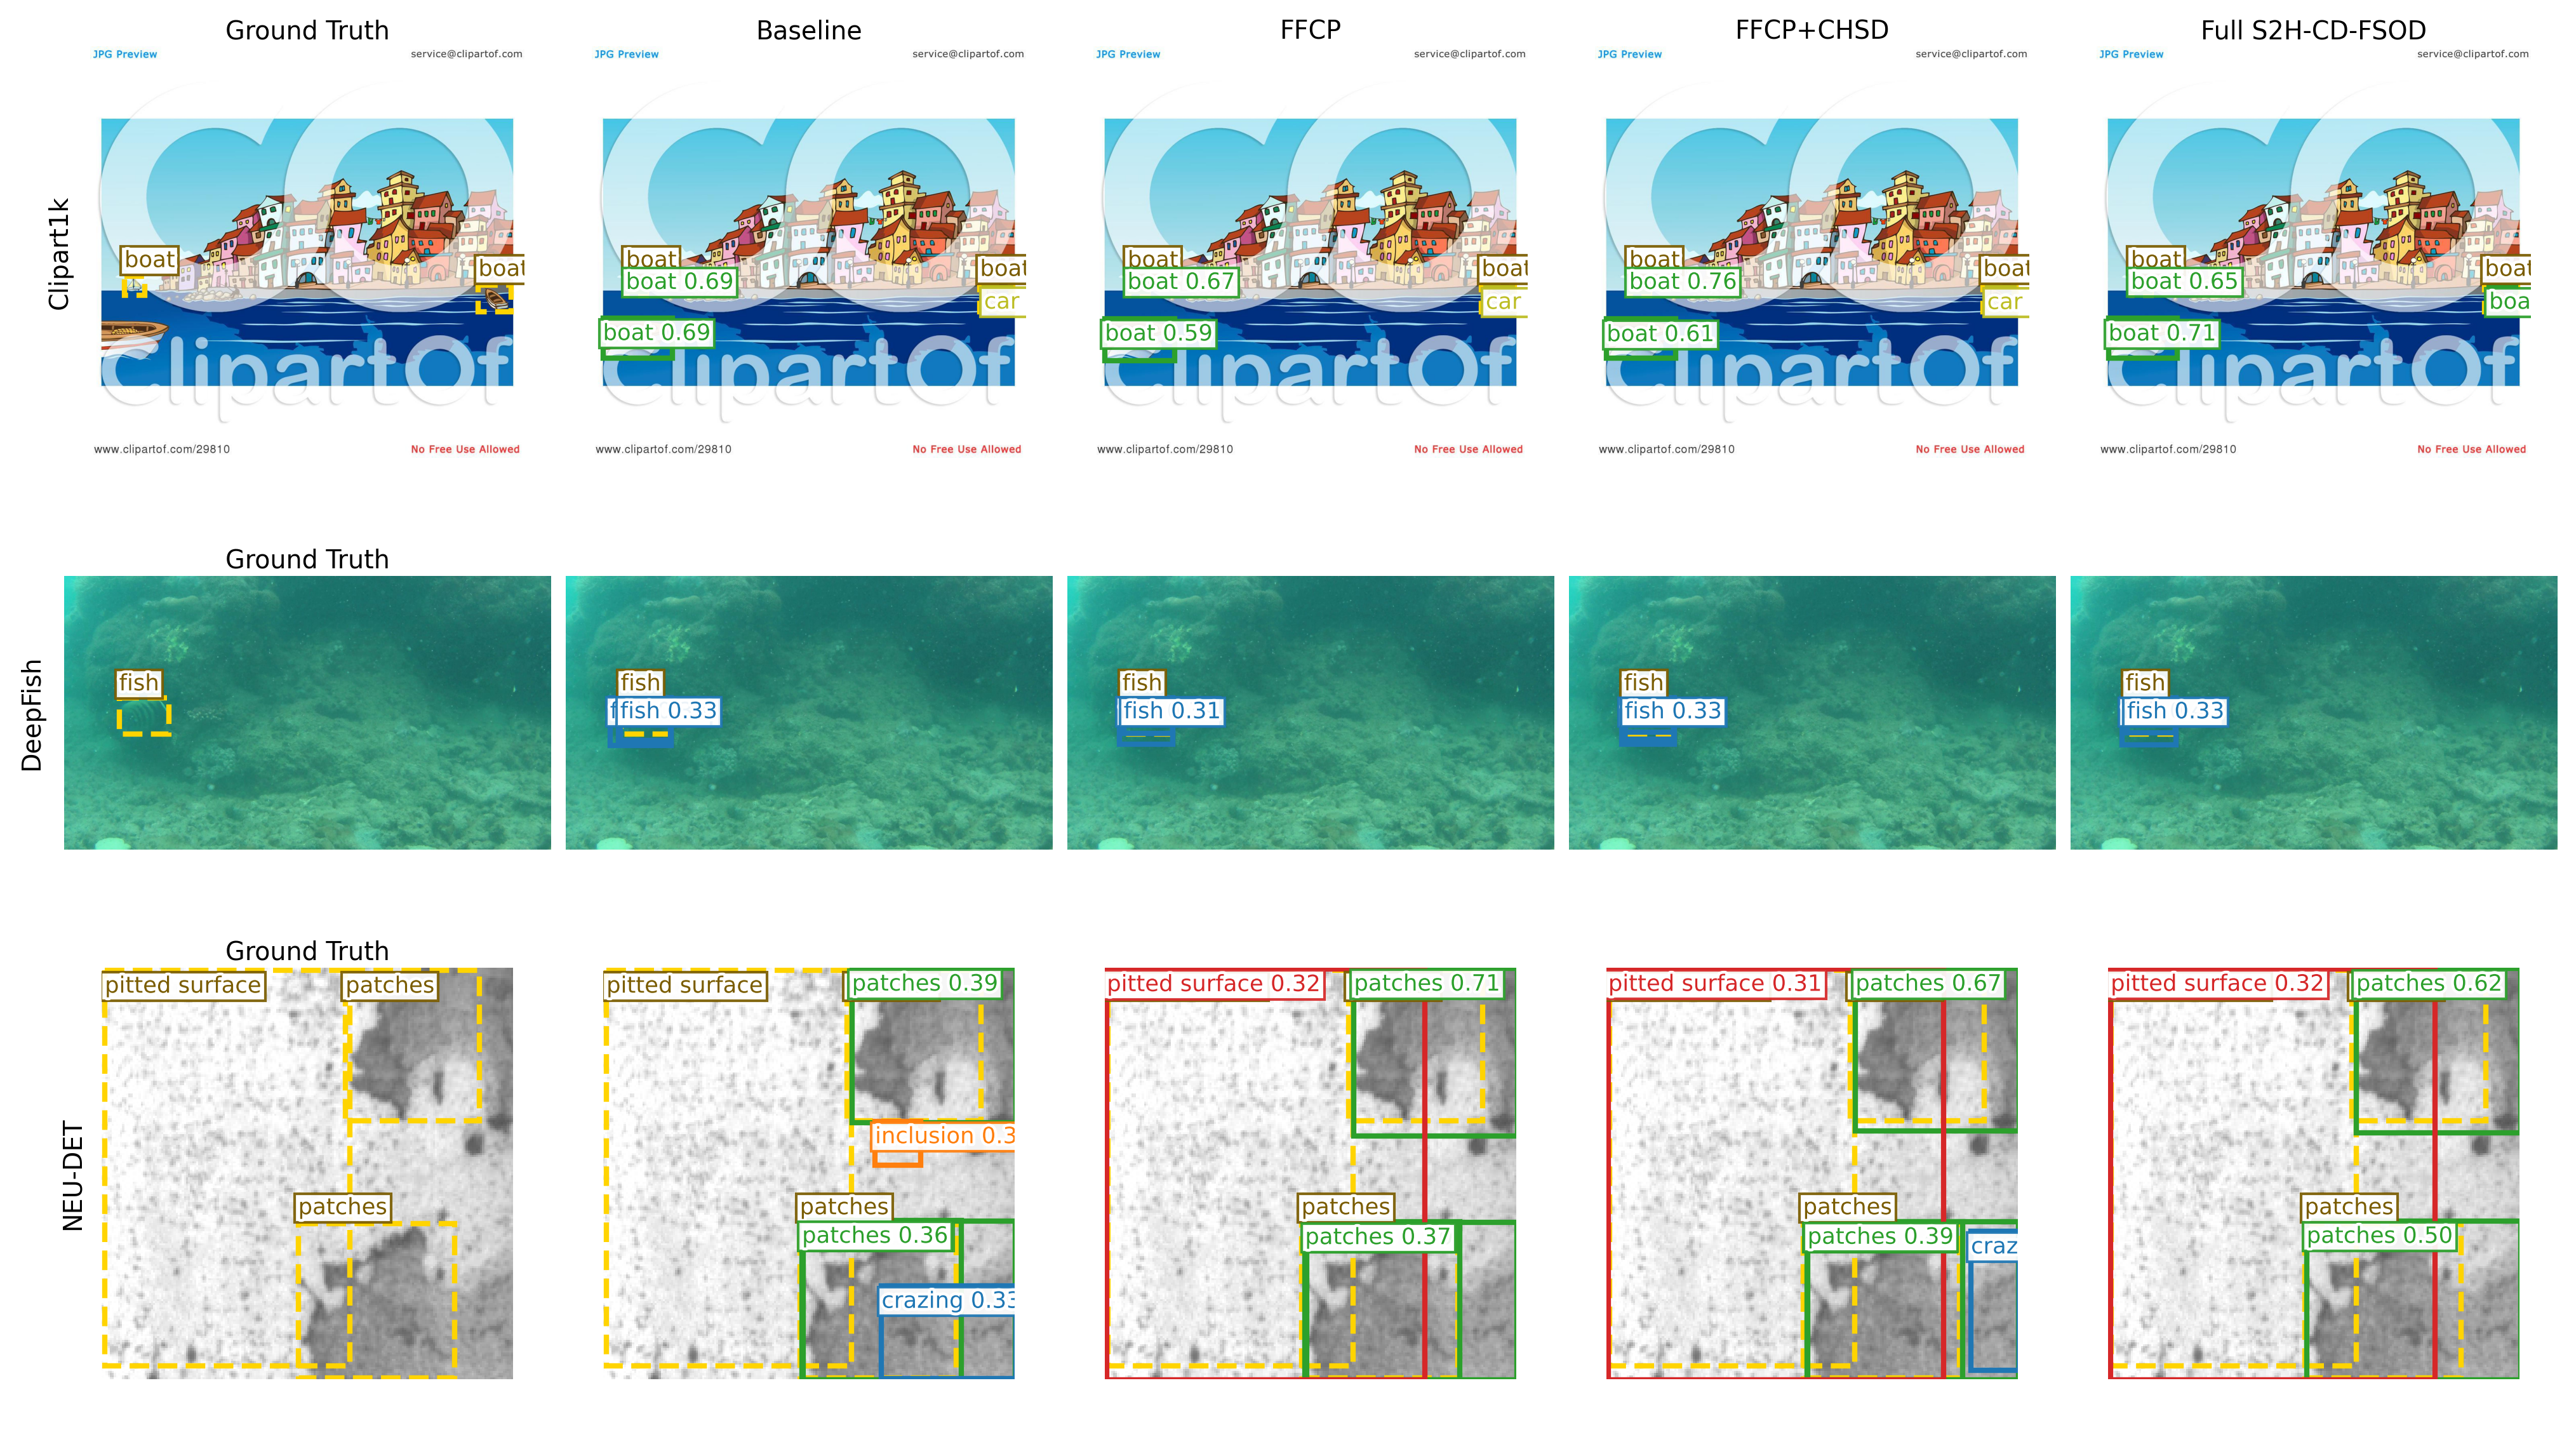
\includegraphics[width=\textwidth]{fig/confidence_progression.png}
    \caption{\textbf{Qualitative detection comparison on 5-shot target domains.}
    Each row shows a representative example from Clipart1k, DeepFish, and
    NEU-DET, while the columns progress from ground truth to the Grounding DINO
    baseline, FFCP, FFCP+CHSD, and the full S2H-CD-FSOD model. Yellow dashed
    boxes indicate annotated objects; colored prediction boxes are labeled with
    the predicted category and confidence score. The examples illustrate how the
    cumulative stages suppress context-driven or spurious responses while
    retaining detections of the target objects, with the largest changes
    occurring in the cluttered underwater and industrial scenes.}
    \label{fig:confidence_progression}
\end{figure*}


We evaluate four cumulative variants under the 5-shot protocol: the fine-tuned
Grounding DINO baseline, FFCP, FFCP+CHSD, and the complete S2H-CD-FSOD model.
All variants share the support splits, optimization budget, and evaluation
code. Fig.~\ref{fig:ablation_map} summarizes the mean mAP of each variant as a
compact cumulative bar group, and Fig.~\ref{fig:confidence_progression}
visualizes the effect of each stage on representative queries. The cumulative
ordering follows the pipeline: FFCP estimates context-sensitive directions,
CHSD builds the identity/appearance decomposition, and ATAR decides how much
authority the retained evidence receives on each query.

Fig.~\ref{fig:ablation_map} reports the quantitative gains for the four
domains with completed ablation runs (Clipart1k, DeepFish, NEU-DET, and UODD);
the baseline bars use the corresponding Grounding DINO$^\dagger$ values from
Table~\ref{tab:main_comparison}, and the remaining bars are the seed-averaged
mAP values of the current run workbook.
AP50 and AP75 are kept in the numerical tables rather than duplicated as plots,
and only completed runs appear.
Fig.~\ref{fig:confidence_progression} presents
qualitative 5-shot comparisons on Clipart1k, DeepFish, and NEU-DET. The
examples show three complementary effects of the cumulative stages:
context-driven duplicate or category responses are reduced, low-contrast target
detections are retained, and industrial defect boxes remain aligned with the
annotated regions. These examples illustrate the kinds of changes measured by
the aggregate results rather than replacing the numerical comparison.

\subsection{Qualitative Analysis}
\label{sec:qualitative}

Following LMP~\cite{lmp}, the main paper keeps a single cross-domain
visualization (Fig.~\ref{fig:confidence_progression}) and defers the remaining
imagery to the supplementary material. The figure uses the same support split,
checkpoint, preprocessing, score threshold, and post-processing for every
column. Clipart1k exposes contextual boat/car confusions, DeepFish stresses a
small low-contrast fish, and NEU-DET contains overlapping defect categories
such as patches, crazing, and inclusions. The intended outcome is a selective
change in error type---fewer context-driven responses and better-supported
category decisions---rather than a blanket increase in the number of
predictions. Cross-domain qualitative comparisons and balanced failure cases
are reported in the supplementary material.

% Keep the normal float flow between Sections 4 and 5.  Do not add a
% `\FloatBarrier` or `\clearpage` here: either command can flush a pending
% figure and create a large blank region in the two-column layout.
\section{Conclusion}
\label{sec:conclusion}

We introduced support-induced context leakage, a phenomenon in which non-category support factors perturb predictions for an unchanged query after few-shot adaptation. A controlled study on Clipart1k and NEU-DET measures classification and localization drift beyond training-seed variation and shows that intervention severity depends on the target domain. Based on this observation, we proposed a knowledge-enhanced Hard-Soft framework: FFCP identifies context-sensitive directions, CHSD separates an identity anchor from context-cleaned target appearance, and ATAR uses their agreement to authorize a bounded correction only for uncertain queries.

Experiments across six CD-FSOD benchmarks evaluate whether regulating support knowledge improves detection accuracy without destabilizing a strong pretrained detector. Rather than being transferred as an unrestricted prototype, target-domain evidence should first be tested, decomposed, and authorized according to its reliability and the uncertainty of the current query. This principle provides a practical route toward reliable vision-language detector adaptation under scarce supervision.

{
    \raggedbottom
    \setlength{\bibsep}{1pt}
    \small
    \bibliographystyle{ieeenat_fullname}
    \bibliography{main}
}

% Build the supplementary material separately when needed.  Keeping it out of
% the main submission prevents a page-number reset and supplementary floats
% from disrupting the CVPR main-paper layout.
% \clearpage
\setcounter{page}{1}
\maketitlesupplementary

\section{Implementation Details}
\label{sec:suppl_impl}

\paragraph{Training augmentation.}
Every image passes through random horizontal flipping and then one of two
paths: a resize to a randomly sampled scale, or a stronger sequence of
resize, random-size crop, and multi-scale resize, matching the
Grounding DINO recipe~\cite{groundingdino}. At inference all augmentations are
disabled and evaluation follows COCO metrics.

\paragraph{Support-side configuration.}
FFCP uses a fixed context rank across domains, and the Hard update radius, the
routing temperature, and the Soft authority budget are shared across the six
benchmarks. The class-wise estimate is shrunk toward a cross-category drift
subspace in the 1-shot regime and receives progressively more weight as the
number of support instances grows.

\section{Additional Quantitative Analysis}
\label{sec:suppl_extra}

\paragraph{Hyperparameter sensitivity.}
Fig.~\ref{fig:hyperparam} in the main paper summarizes the sensitivity of the
five shared hyper-parameters on 5-shot Clipart1k; the complete per-value sweep
tables are provided in the released code. Each sweep varies one quantity while
keeping the support split, checkpoint, and optimization budget fixed, and the
shared cross-domain configuration is selected from the central stable region
rather than tuned per domain.

\section{Additional Qualitative Analysis}
\label{sec:suppl_qual}

\paragraph{Cross-domain qualitative comparison.}
Fig.~\ref{fig:qualitative_six_domains} shows one representative query per
target domain, with the ground truth, the text-only baseline, and the full
model as columns. Both methods share the support split, checkpoint,
preprocessing, score threshold, and post-processing.

\begin{figure*}[t]
    \centering
    \includegraphics[width=0.72\textwidth]{fig/qualitative_six_domains.png}
    \caption{Qualitative comparison across six CD-FSOD target domains in the
    5-shot setting. Each row is one domain; columns are the ground truth, the
    text-only Grounding DINO baseline, and the full S2H-CD-FSOD model.}
    \label{fig:qualitative_six_domains}
\end{figure*}

\paragraph{FFCP interventions.}
Fig.~\ref{fig:intervention_examples} visualizes the foreground-frozen
interventions that produce the context-sensitive directions used by CHSD. Each
ground-truth box is accompanied by jittered regions at increasing overlap with
the object, which retain realistic partial-object and boundary cues while
changing the surrounding context. These views expose the neighboring objects
and domain-specific background patterns that drive false positives, and explain
why the context-sensitive subspace is removed from the identity anchor.

\begin{figure*}[!t]
    \centering
    \includegraphics[width=0.6\textwidth]{fig/intervention_examples.png}
    \caption{Foreground-frozen interventions across six target domains. Each row
    shows the protected ground-truth box and several jittered regions that change
    only the surrounding context. These probes identify where external context
    perturbs the otherwise unchanged target representation.}
    \label{fig:intervention_examples}
\end{figure*}

\paragraph{Failure cases.}
Fig.~\ref{fig:failure_cases} retains representative failures so that the
qualitative analysis is not reduced to successful examples: severe occlusion,
very small objects, atypical support prototypes, and residual false positives
in the full model. Authority routing mitigates support-induced errors but does
not remove the intrinsic ambiguity of an underspecified support set.

\begin{figure*}[t]
    \centering
    \includegraphics[width=\textwidth]{fig/failure_cases.png}
    \caption{Representative failure cases. Red boxes mark false positives,
    yellow dashed boxes mark missed ground truths, and purple labels mark
    incorrect category assignments.}
    \label{fig:failure_cases}
\end{figure*}




\end{document}
